\chapter{Diseño e implementación}

En esta sección explicamos en detalle los productos que hemos desarrollado para los científicos Israelíes. Hemos partido de un dataset facilitado por ellos, que hemos utilizado para entrenar un modelo que genera imágenes sintéticas y para implementar un clasificador de imágenes.

Toda la implementación se encuentra en el repositorio de GitHub del proyecto \cite{repository}. La raíz del repositorio contiene los siguientes elementos:

\dirtree{%
    .1 /.
    .2 experiments/\DTcomment{implementación del TFG}.
    .2 papers/\DTcomment{algunas de las publicaciones utilizadas en su desarrollo}.
    .2 report/\DTcomment{memoria en formato \LaTeX}.
    .2 slides/.
    .2 README.md.
}

\section{Dataset utilizado}
El dataset contiene ejemplos positivos y negativos. Todas las imágenes son diferentes, presentan elementos con distintos trazados de línea, tamaños, colores... Originalmente se encuentran en formato .png.

Los ejemplos positivos son imágenes de moléculas extraídas de publicaciones. La mayoría son moléculas completas, aunque algunas parecen recortes de estructuras más grandes. En total tenemos 162 imágenes de este tipo.

\begin{figure}[H]
\centering
    \fbox{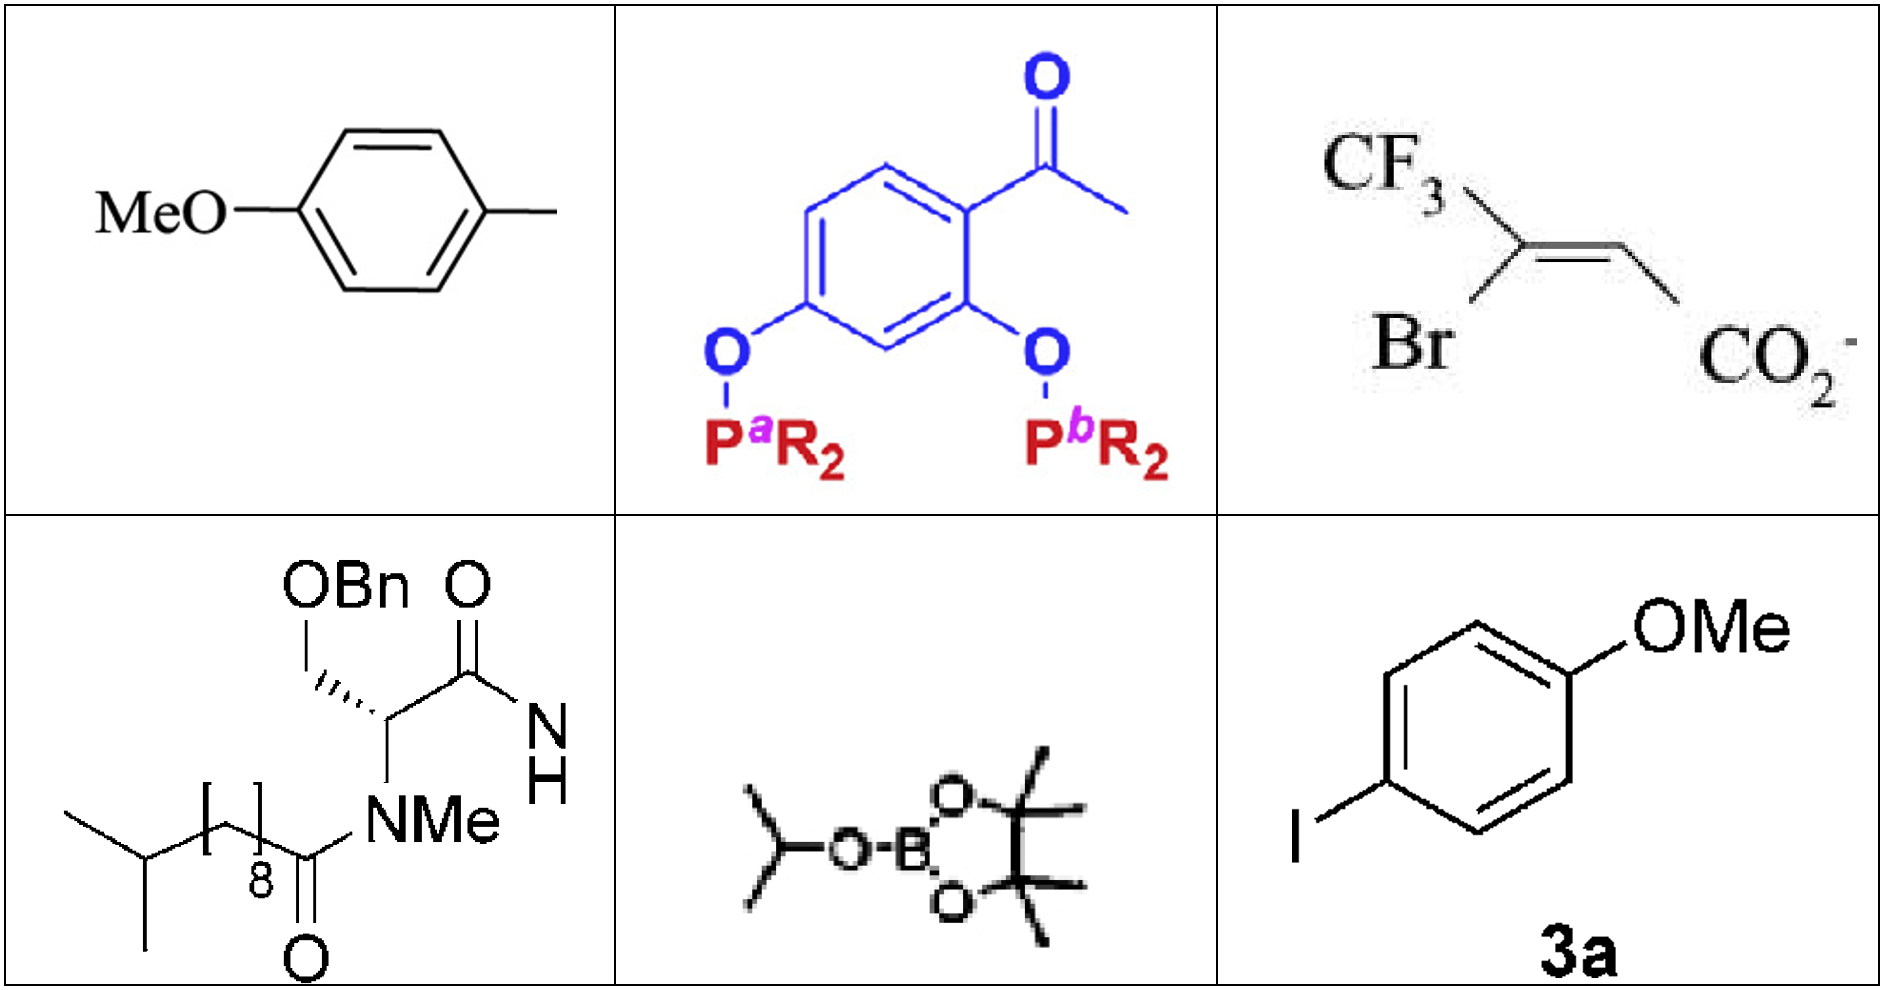
\includegraphics[scale=0.3]{imagenes/positive_examples.png}}  
    \caption{Ejemplos de muestras positivas del dataset} 
\end{figure}

Los ejemplos negativos son, en cambio, imágenes que contienen rectas, curvas y otras figuras que se parecen a las formas que adquiere una molécula, pero no lo son. En esta categoría hay muchas más imágenes, 800 en total.

\begin{figure}[H]
\centering
    \fbox{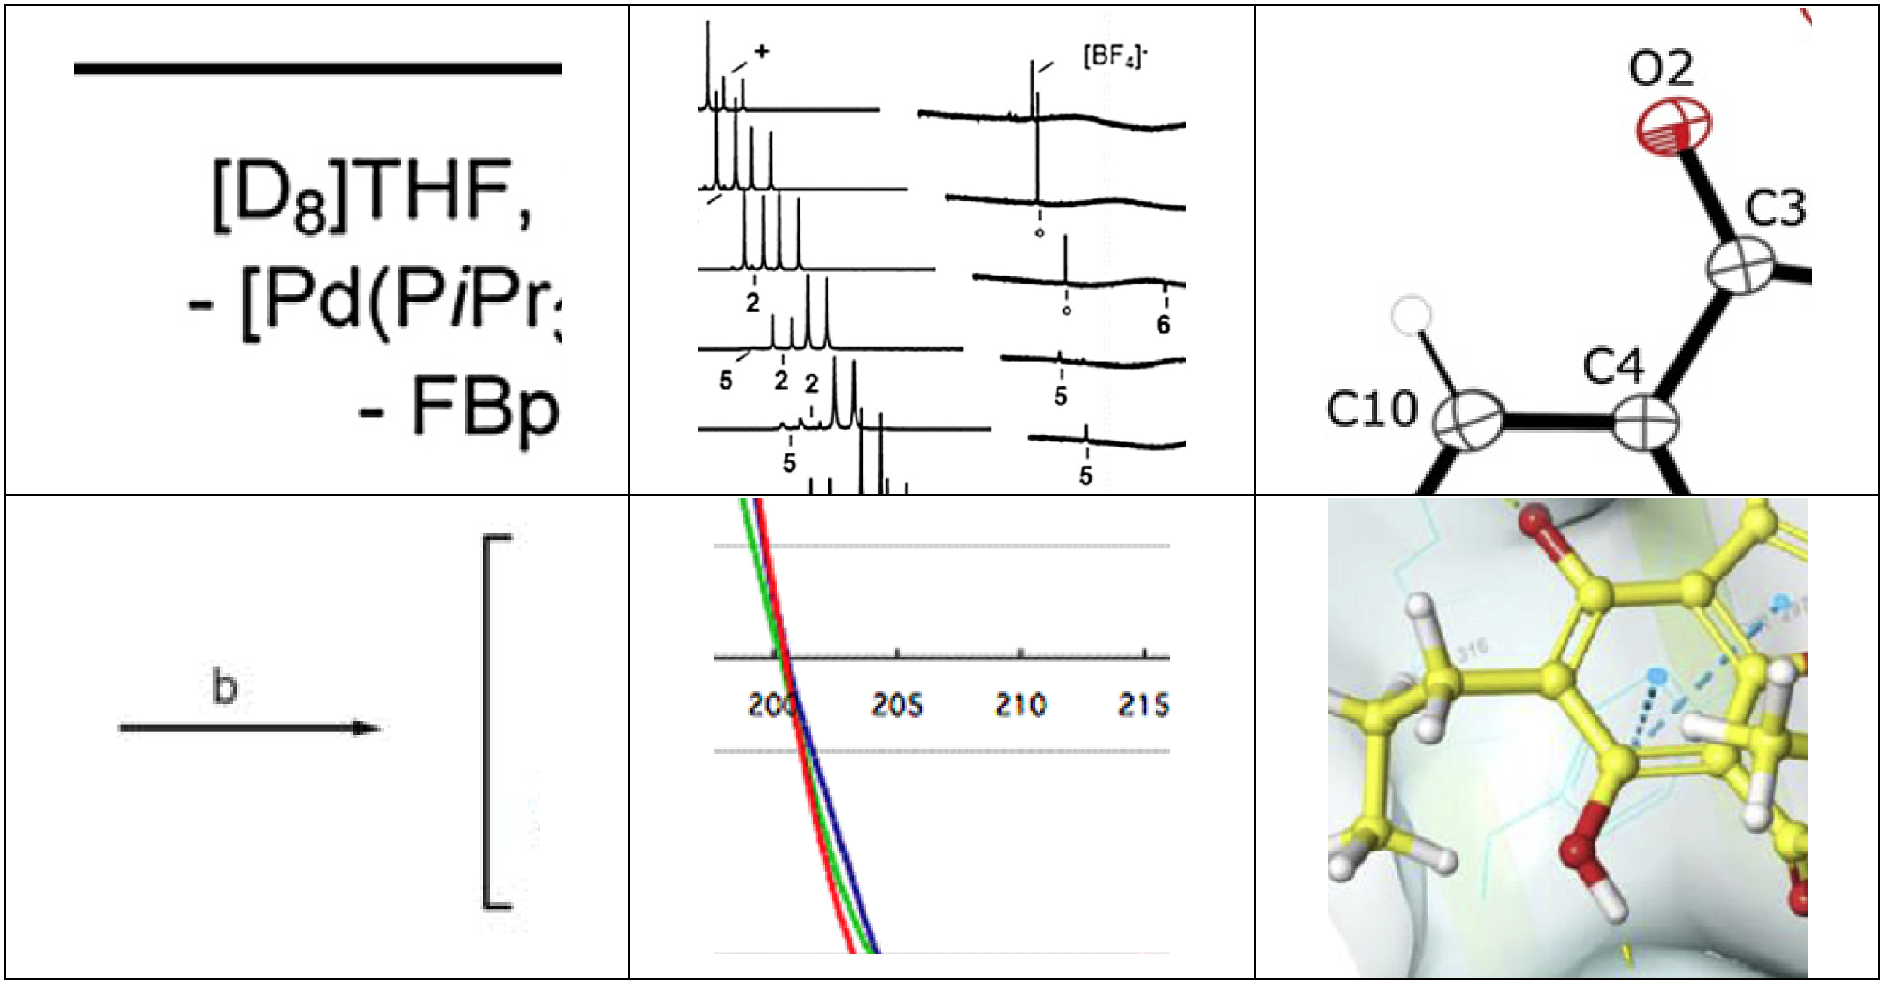
\includegraphics[scale=0.3]{imagenes/negative_examples.png}}  
    \caption{Ejemplos de muestras negativas del dataset} 
\end{figure}

Estas imágenes necesitan un preprocesamiento, es necesario elegir el formato con el que se va a trabajar y dimensionarlas para que todas tengan el mismo tamaño. Debido a que el canal alfa del formato .png no se está aprovechando, decidimos convertirlas a formato .jpg y así trabajar con tres canales en nuestros modelos. Además, el modelo generador que utilizamos está diseñado para trabajar con imágenes con este número de canales, así que será lo más adecuado.

También mencionar el limitado número de ejemplos positivos que tenemos en comparación con negativos. Ya que los modelos de Deep Learning aprenden mejor cuantos más datos existen, vamos a aumentar su número. Para ello, vamos a aplicar una serie de transformaciones sobre las imágenes originales, de forma que sean parecidas pero se encuentren rotadas, estiradas, con cierto grado de ruido gaussiano, etc. Aunque en algunos casos haremos pruebas con otras secuencias de transformaciones, la mayoría de experimentos los llevaremos acabo utilizando datos generados mediante la siguiente secuencia:

\begin{algorithm}[H]
    \caption{aug2: secuencia de data augmentation aplicada }
\begin{algorithmic}
    \State Prueba
\end{algorithmic}
\end{algorithm}



\section{Estructura del código}
Como se menciona al principio del capítulo, la implementación se sitúa en el directorio $experiments/$, dividido en dos subdirectorios. El primero contiene el código del modelo generador de imágenes, el segundo el del clasificador: \\

\dirtree{%
    .1 experiments/\DTcomment{implementación del TFG}.
    .2 taming\_transformers/\DTcomment{generador de imágenes}.
    .3 taming-transformers/.
    .4 configs/.
    .4 logs/.
    .4 train\_ngpu.sh.
    .3 data\_generation\_and\_aug.ipynb.
    .3 sample\_and\_clean\_molecules.ipynb.
    .3 sampling\_experiment.ipynb.
    .3 functions.py.
    .2 image\_classifier/\DTcomment{clasificador de imágenes}.
    .3 saved\_models/.
    .3 datasets.py.
    .3 functions.py.
    .3 grid\_search.py.
    .3 models.py.
    .3 train.py.
    .3 train\_ngpu.sh.
}

\subsection{Generador de imágenes sintéticas}
Uno de los objetivos del proyecto es construir un modelo que nos permita generar imágenes sintéticas de moléculas. 

\section{Ejecución y reproducibilidad}
Como ejecutar los scripts y semillas utilizadas